\subsection{\textcolor{red}{Используемый в работе подход}}
    В качестве подхода, на основе которого строится решение задачи по установлению связей между твитами и новостями, был выбран WTMF-G.
    Основной причиной подобного выбора является то, что большинство подходов учитывают только статистические зависимости вида текст-слово;
    метод WTMF-G, напротив, не ограничивается зависимостями текст-слово, а позволяет учесть взаимосвязь текст-текст,
    что, как ожидается, даст прирост качества в решении задачи установления связей.

    Также, в рамках работы задача по установления связей между твитами и новостями решена классическим подходом для установления связей между текстами~---~
    определение схожести текстов на основе частотности употребления слов. Этот подход даёт хорошие результаты на больших текстах.
    Результаты этого метода помогут оценить влияние связей вида текст-текст в методе WTMF-G на качество полученного решения.

    Ниже представлено описание теории, необходимой для реализации метода WTMF-G.

    \subsubsection{Построение набора данных}
        Для решения задачи автоматического связывания твитов и новостей необходимо иметь эталонный набор данных, на котором будет производится оценка качества полученного решения.

        Сначала за общий период времени собираются твиты и новости.
        Для твита помимо текста хранится информация о времени публикации и авторе работы. Для новости хранится время публикации, заколовок, краткое изложение и URL.

        На основе собранной информации строится набора данных, который состоит из трёх частей:
        \begin{enumerate}
            \item множество новостей~---~все собранные новости;
            \item множество связей твит-новость, под связью подразумевается явное указание URL новости в тексте твита;
            \item множество твитов~--~все твиты, имеющие связь с одной из собранных новостей.
        \end{enumerate}
    \subsubsection{Метод WTMF}
    \label{subsubsec:wtmf}
        Метод WTMF учитывает отсутствующие в тексте слова в виде признаков короткого текста.
        Под отсутствующими словами подразумеваются все слова из корпуса, составленного из всех текстов, за исключением слов из рассматриваемого короткого текста.
        То есть отсутствующие слова можно трактовать как негативный сигнал.

        Работа метода WTMF основана на разложении TF-IDF матрицы $X$ в произведение двух матриц $P$ и $Q$:
        $$X \sim P^TQ.$$
        На рисунке~\ref{pic:wtmf} показано как матрица $X$ приближается произведением двух матриц $P^T$ размера $M \times K$ и $Q$ размера $K \times N$.

        \begin{figure}[h!]
            \center
            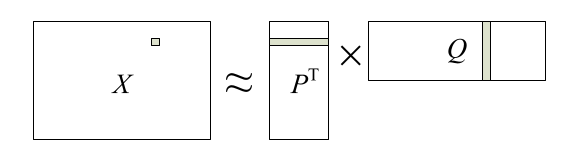
\includegraphics[scale=0.45]{wtmf.png}
            \caption{Разложение TF-IDF матрицы~($X$) на произведение матриц $P$ и $Q$}
            \label{pic:wtmf}
        \end{figure}

        Каждый текст $s_j$ представлен в виде вектора $Q_{\cdot,j}$ размерности $K$, каждое слово $w_i$ представлено в виде вектор $P_{i,\cdot}$.
        Если $X_{ij}=(P_{i,\cdot}, Q_{\cdot,j})$ близко к нулю, то это трактуется как отсутствующее слово.

        Задачей метода является минимизация целевой функции ($\lambda$ - регуляризирующий член, матрица W определяет вес элементов матрицы X):
        $$\sum_i \sum_j W_{ij} (P_{i,\cdot} \cdot Q_{\cdot,j} - X_{ij})^2 + \lambda ||P||^2_2 + \lambda ||Q||^2_2.$$

        Для получения векторов $P_{i,\cdot}$ и $Q_{\cdot,j}$ используется алгоритм описанный в статье~\cite{matrix_approximation}.
        Сначала P и Q инициализируются случайными числами. Затем запускается итеративный пересчёт P и Q по следующим формулам (эффективный способ расчёта описан в \cite{steck_recommender}):
        $$P_{i, \cdot} = (Q W'_i Q^T + \lambda I)^{-1} Q W'_i X_{i,\cdot}^T,$$
        $$Q_{\cdot, j} = (P W'_j P^T + \lambda I)^{-1} P W'_j X_{j,\cdot}.$$
        Здесь $W'_i = diag(W_{i, \cdot})$ - диагональная матрица полученная из $i$-ой строчки матрицы $W$,
        аналогично $W'_j = diag(W_{\cdot, j})$ - диагональная матрица полученная из $j$-ого столбца матрицы $W$.
        Матрица $W$ определяется следующим образом:
        \begin{gather}
            W_{ij} =
            \begin{cases}
                1, ~~if~X_{ij} \neq 0, \nonumber \\
                w_m, ~~otherwise.
            \end{cases},
        \end{gather}
        где $w_m$ положительно и $w_m << 1$.

        Столбцы построенной матрицы Q представляют собой вектора для сравнения текстов между собой.
        Тексту, на основе которого построена $i$-я строка TF-IDF матрицы $X$, в соответствие ставится $i$-й столбей матрицы Q.

    \subsubsection{Построение связей текст-текст}
    \label{subsubsec:linking}
        Построение связей текст-текст предполагает поиск потенциально семантически близких текстов.
         При построении связей текст-текст используются три способа:
        \begin{enumerate}
            \item построение связей на основе общих хэштегов,
            \item построение связей на основе общих именованных сущностей,
            \item построение связей на основе близости по времени.
        \end{enumerate}

        \paragraph{Связь твитов с помощью хэштегов.}
            Из твитов извлекаются все хэшетеги.
            Затем в хэштеги превращаются все слова во всех твитах, которые совпали с ранее извлечёнными хэштегами.
            Для каждого твита и для каждого хэштега извлекается $k$ твитов, которые содержат этот хэштег.
            Если хэштег появлялся в более чем $k$ твитах, то берём $k$ твитов наиболее близких во времени к исходному.

        \paragraph{Связь твитов с помощью именованных сущностей.}
            К краткому изложению новостей применяются методы извлечения именованных сущностей.
            Для каждого твита, содержащего именованную сущность в виде отдельного слова извлекается $k$ твитов, которые содержат эту же именованную сущность.
            Если именованная сущность содержалась более чем в $k$ твитах, то берём $k$ твитов наиболее близких во времени к исходному.

        \paragraph{Связь твитов и новостей на основе близости по времени}
            Для каждого твита~(новости) выбираем $k$ связей с наиболее схожими твитами~(новостями) в окрестности 24 часов.
    \subsubsection{Метод WTMF-G}
        Метод WTMF-G~(WTMF on Graphs)~---~ представляет собой метод WTMF, расширенный путём добавления связей текст-текст.
        Добавление связей текст-текст происходит путём модификации регуляризирующего члена $lambda$. Для каждой пары связанных текстов $j_1$ и $j_2$:
        $$\lambda = \delta \cdot (\dfrac{Q_{\cdot,j_1}\cdot Q_{\cdot,j_2}}{|Q_{\cdot,j_1}|| Q_{\cdot,j_2}|}-1)^2,$$
        коэффициент $\delta$ задаёт степень влияния связей текст-текст.

        Так как новый регуляризирующий член $lambda$ зависит от $|Q_{\cdot,j}|$, который меняется во время итерации, вводим упрощение: длина вектора $Q_{\cdot,j}$ не изменяется во время итерации.
        Также необходимо модифицировать итеративный процесс построения матриц $P$ и $Q$ следующим образом:
        $$P_{i, \cdot} = (Q W'_i Q^T + \lambda I)^{-1} Q W'_i X_{i,\cdot}^T,$$
        $$Q_{\cdot, j} = (P W'_j P^T + \lambda I + \delta  L_j^2 Q_{\cdot,n(j)} diag(L^2_{n(j)})Q_{\cdot,n(j)}^T)^{-1}   (P W'_j X_{j,\cdot} + \delta  L_j Q_{\cdot,n(j)} L_{n(j)}).$$
        В этих формулах $n(j)$~---~список связанных текстов с текстом $j$. $Q_{\cdot,n(j)}$~---~матрица, состоящая из связанных векторов для $Q_{\cdot, j}$.
        $L_j$ - длина вектора $Q_j$ на начало итерации, $L_n(j)$~---~вектор длин векторов связанных с $j$, то есть $Q_{\cdot,n(j)}$, полученный на начало итерации.
